\documentclass[main.tex]{subfiles}
\begin{document}
\chapter{Introduction}
%------------------
%------------------
\section{Motivation}
Modern robotic systems are designed as {underactuated} systems. These systems feature more degrees of freedom in the movement of the joints than there are actuators controlling their motions\cite{underactuated}. 
For robots with two or more degrees of underactuation, the dynamics may become highly complex. In fact, underactuated dynamics are often not even Euler-Langrange\cite{mccarthy}.
\begin{figure}[H]
    \centering
    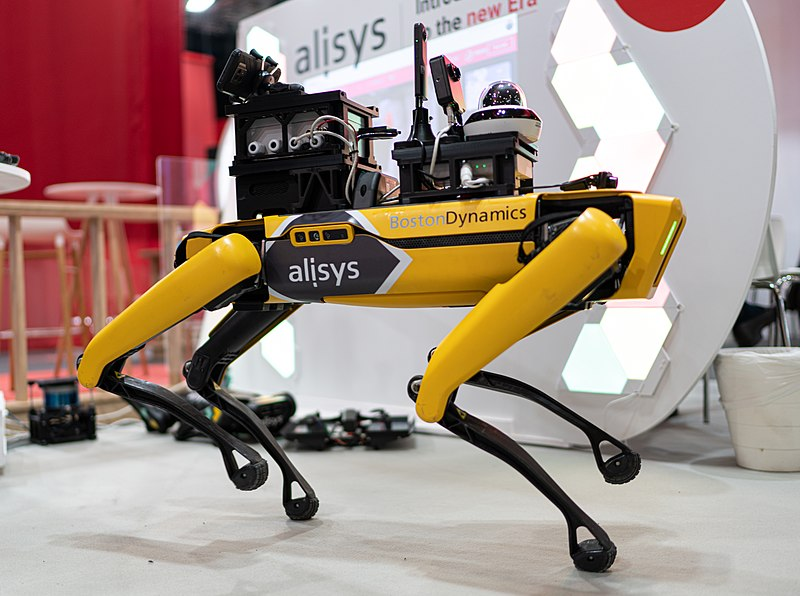
\includegraphics[width=0.5\textwidth]{assets/bostondyn.png}
    \caption{A Boston Dynamics four-legged robot demonstrates its ability to balance in 2021 \cite{bostondyn}}
    \label{fig:bostondyn}
\end{figure}
It is therefore necessary to have a suite of fast, reliable methods for analyzing and controlling these underactuated robots. One approach is called dyamical reduction, wherein complex dynamics are simplified using mathematical techniques. Modeling a system to be with only a subset of its generalized coordinates, without compromising on the usefulness and accuracy of the model, allows for faster and more efficient computation and control.
\section{Overview}
This project explores the behaviour of some simple, underactuated, mechanical control systems endowed with symmetry subjected to virtual holonomic constraints (VHCs). 

The chosen systems feature at least one Lagrangian symmetry, and two degrees of underactuation. Each actuator is made to enforce a VHC that respects the symmetry of the system--in other words, the system is controlled to maintain a particular configuration whose Lagrangian is invariant.

Each system is modelled in the Lagrangian formulation using Matlab. A suitable VHC is chosen, and then the constrained dynamics are derived using parametrization in terms of the VHCs. The constrained dynamics are also derived using Christoffel symbols--both methods should agree.

\section{Notation}
\begin{enumerate}[(1)]
    \item\label{def:jacobian} $\dd f_q$ is the Jacobian operator with respect to the coordinates $q$, applied to the vector function $f(q)$. Explicitly:
    \begin{align}
        f&:=\Vec{f}(\Vec{q}),\\
        \dd f_q&:= \pdv{f^i}{q^j}\hat{e}_i\cdot\hat{e}^\top_j.
    \end{align}
    \item $A^\top$ is the transpose of the matrix $A$, explicitly $[A^\top]_{ij}=[A]_{ji}$.
    \item $\Ker{A}$ is the kernel, or nullspace, of a matrix $A$. Explicitly, the solution set $\cbr{x\in\ree^n:Ax=0_n}$.
    \item $T_qQ$ is the tangent space of a point $q$ on the manifold $Q$. By extension, $TQ$ is the tangent bundle given by $TQ:=\bigsqcup_{q\in Q} T_qQ.$
    \item $\Gamma^k_{ij}$ is the $(i,j,k)$\textsuperscript{th} Christoffel Symbol of the Riemannian metric, as defined in Equation \ref{eq:christoffel}.
    \item $\Gammac{k}{ij}$ is the $(i,j,k)$\textsuperscript{th} Christoffel Symbol of the constrained dynamics metric, as defined in Equation \ref{eq:christoffelconstrained}.
    \item $B^\bot$ is the left-annihilator of the matrix $B$, so that $B^\bot B=0$.
\end{enumerate}

\end{document}